\chapter{\textbf{Padrão Publish/Subscribe}} % Este comando é utilizado para criar capítulos

A constante evolução da Internet das coisas (IoT) força, consequentemente, a evolução no contexto de redes e arquiteturas de computadores. A crescente de dispositivos IoT ligados à rede está aumentando exponencialmente ao decorrer dos anos, segundo \cite{7263372}, uma estimativa feita em 2015 para o número de dispositivos IoT implementados na internet é na ordem de 50 bilhões, em 2020, a estimativa é 1000 vezes em relação a 2015 de dispositivos IoT conectados. Isso só se torna possível com a implementação de novos padrões de arquiteturas de redes, que consequentemente, a possibilidade de implementar larga escala de dispositivos IoT, pois oferecem melhor custo benefício, eficiência energética se comparado a padrões antigos.\par

A utilização de abstrações mais naturais e simples é essencial para um contexto das redes dos dispositivos IoT. A ideia inicial de um padrão Publish/Subscribe é sugerida por \cite{Birman1987}, que visa uma implementação de redes em sistemas distribuídos de forma mais natural e que exista a possibilidade de alta escala.\par


Para um melhor entendimento do padrão publish/subscribe, primeiro precisamos definir o conceito largamente utilizado em soluções web, o Request-response. Segundo \cite{Luoto2018}, uma comunicação utilizando o padrão request-response, temos, em princípio dois atores, o cliente, qual irá requisitar os dados, e o servidor, que fará a parte de disponibilizar os recursos solicitados pelo cliente, como podemos observar na figura 1.\par



\begin{figure}[H]
    \centering
	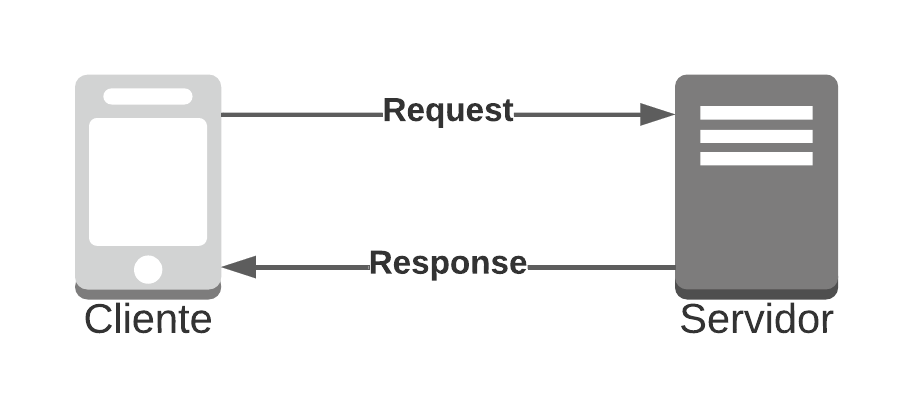
\includegraphics[scale=0.95]{topics/reqres.png}
	\caption{Esquema de requisição-resposta de uma informação. Fonte: o autor.}
\end{figure}


Neste padrão, o servidor sempre aguarda as requisições que podem chegar dos clientes, entretanto, uma conexão é estabelecida temporariamente com o servidor, e após que as requisições forem respondidas, o pedido é dado concluído e não existe conexão posterior com servidor.\par
O padrão Observer também possui dois atores principais, os observadores (Observer) e sujeitos (Subject). Esses atores atuam diretamente na forma de exposição ao dado, qual, o observador, realiza uma requisição de inscrição em determinado sujeito, e dessa forma, ele passa a ser notificado quando existir alguma mudança de estado. O sujeito irá possuir uma lista com os observadores, possibilitando o envio das notificações somente quando houver alguma mudança no sujeito, observável na figura 2.\par

\begin{figure}[H]
    \centering
	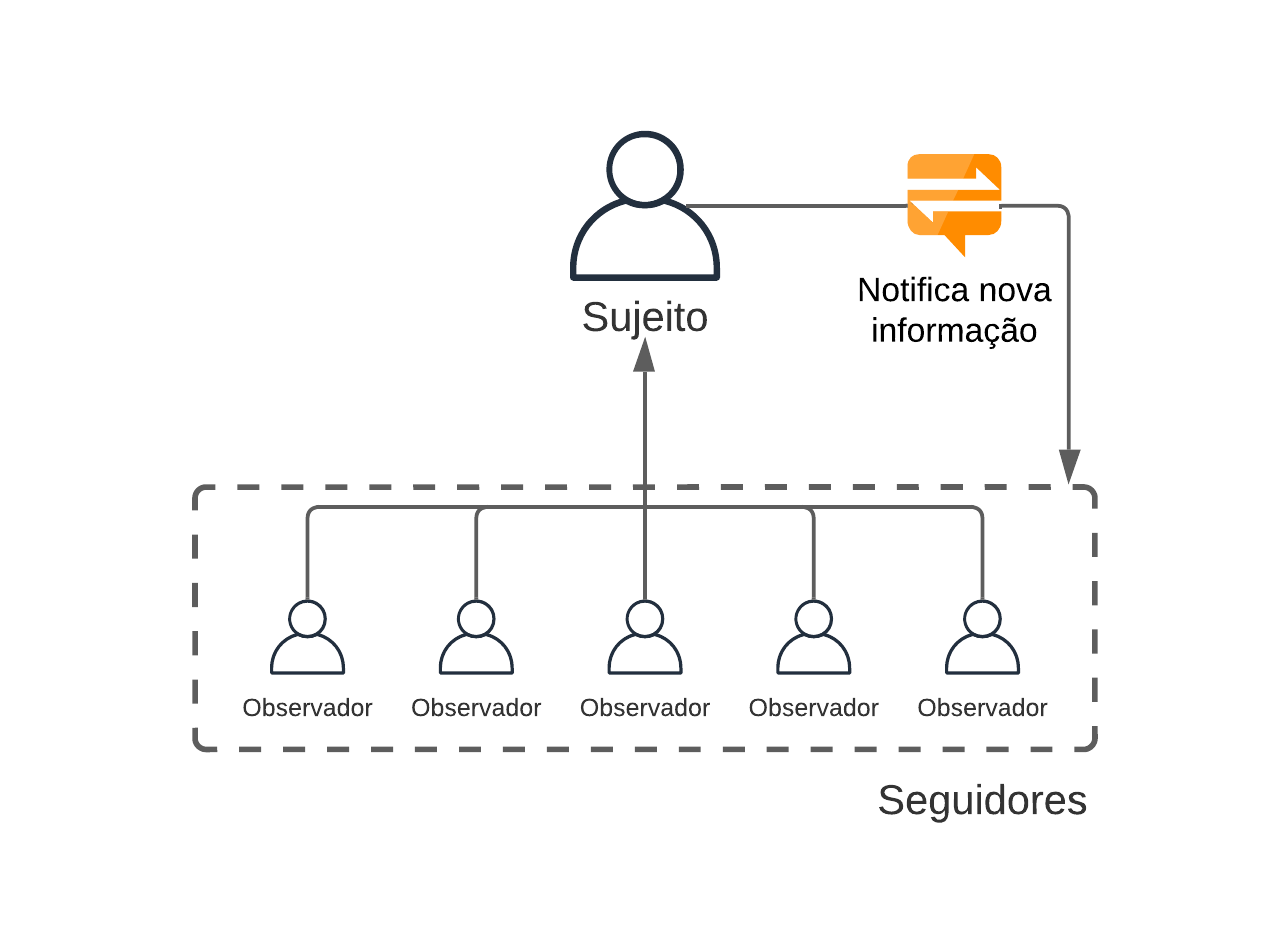
\includegraphics[scale=0.98]{topics/observer.png}
	\caption{Publicação de notificação em esquema Observer. Fonte: o autor.}
	\label{fig:observer}
\end{figure}

Contudo, o padrão publish/subscribe, proposto por \cite{Birman1987}, possui semelhanças com o padrão de observador, neste caso,os atores semelhantes são o publicador (Publisher), responsável por publicar determinada informação em um tópico específico, o inscritos (Subscribe) que ingressa em determinado tópico que receberá notificações das publicações, esquematizado pela figura 3.\par

\begin{figure}[H]
    \centering
	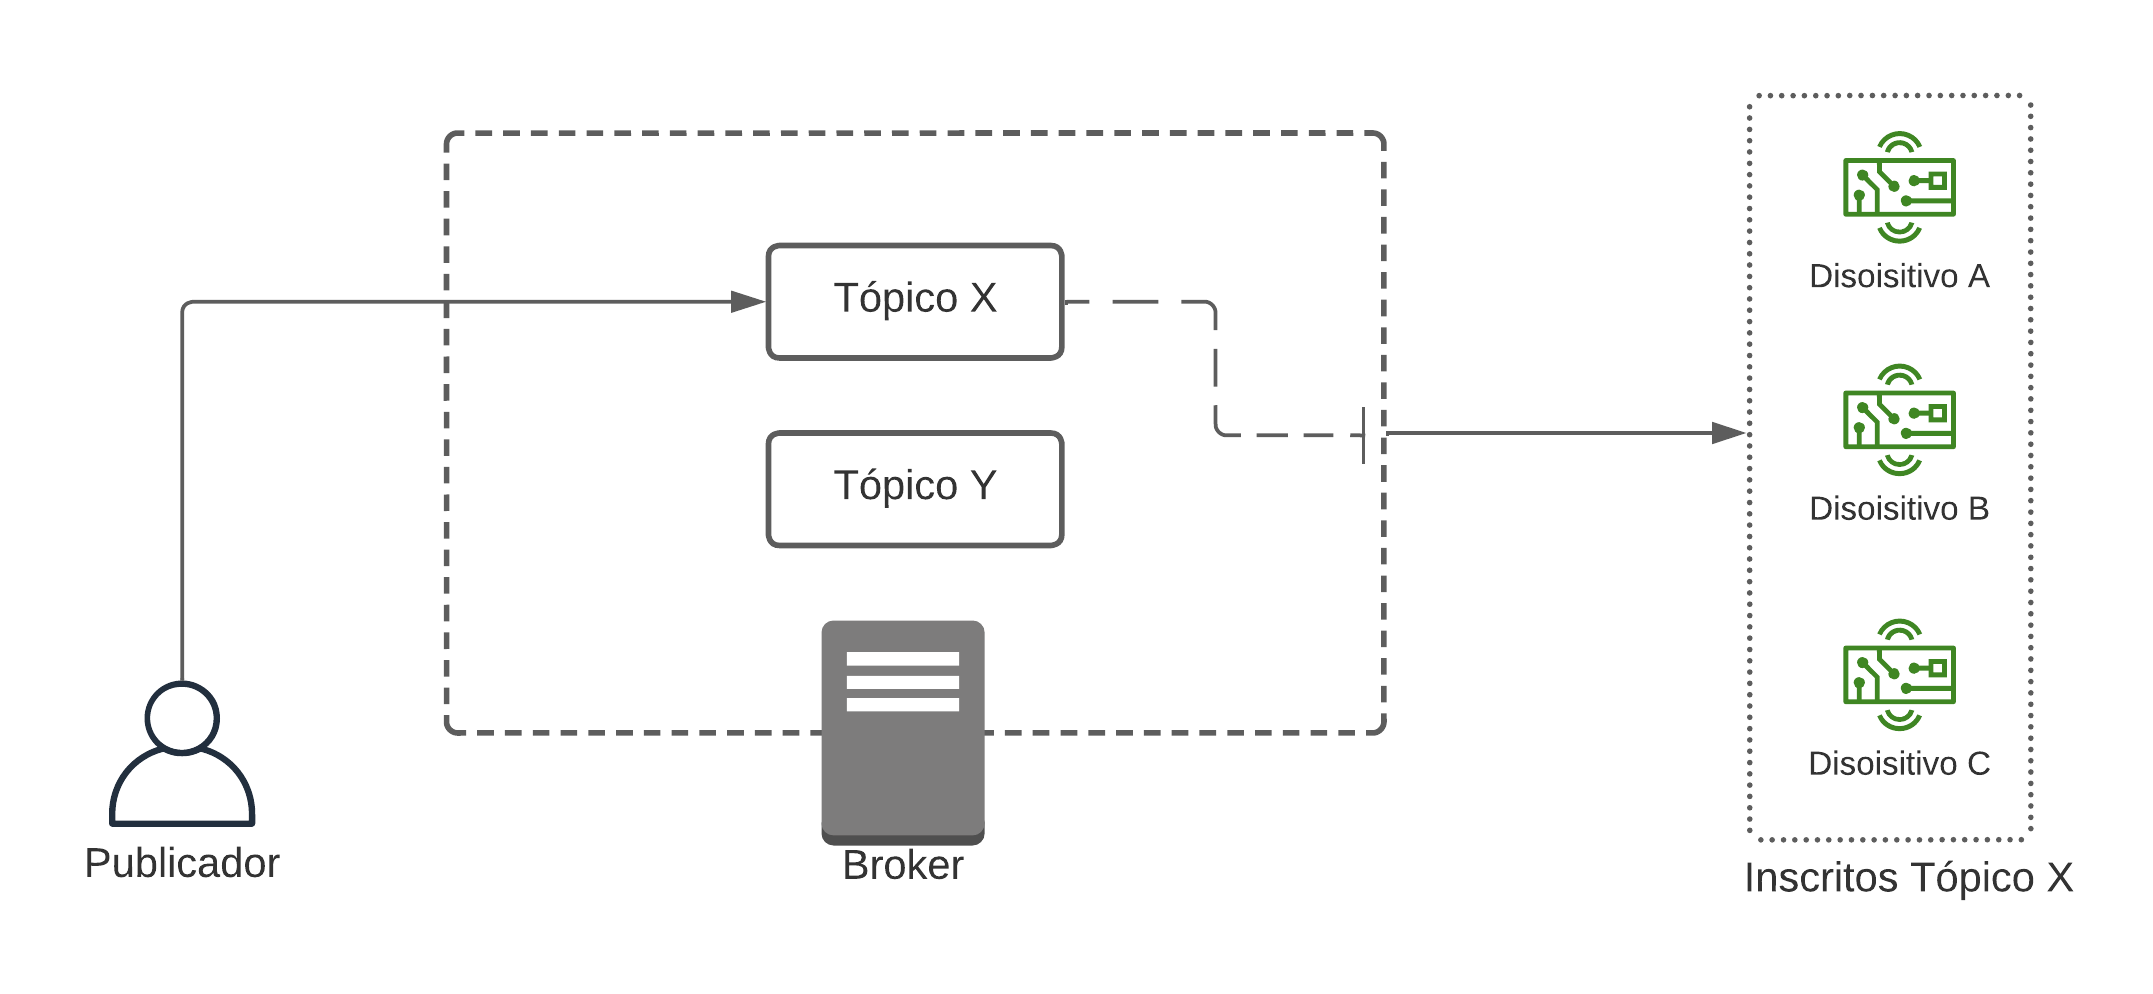
\includegraphics[scale=0.90]{topics/pubsub.png}
	\caption{Esquema de publicação no padrão publish/subscribe. Fonte: o autor.}
	\label{fig:pubsub}
\end{figure}

Entretanto, o novo autor, o Broker, ficará responsável por manipular as notificações a serem enviadas do publicador ao inscritos. Dessa forma, os atores não precisam, necessariamente, terem um contato direto, ou ao menos se conhecer, pois tudo é intermediado pelo Broker, que fará a notificação de mudança dos estados e as informações a serem enviadas para os inscritos no tópico. O Publicador é responsável somente pelo envio das informação a ser distribuida, estabelecendo conexão única e direta ao Broker.

